\documentclass[aps, superscriptaddress, groupedaddress, preprint]{revtex4}

\usepackage{amssymb}
\usepackage{amsmath}
\usepackage{float}
\usepackage{graphicx}

\renewcommand\vec{\mathbf}


\begin{document}

\tableofcontents

\section{Model}


\subsection{Atoms}

Atoms move ballistically.  Emitted from an oven at a temperature
$T$ with mean velocity $\bar{v}$.  Collimated to an angle
$\alpha$ in direction transverse to beam.  With flux $\dot N$,
density $\rho$.

We model them with particles of weight $w$, meaning that a
particle in the simulation corresponds to $w$ real particles.
There is an assumption here about how the dipoles due to the
different atoms add up: Coherent addition.  Good above threshold
but needs to be verified by scaling $w$ down.


\subsection{Atom-Field interaction}

The internal state of the atoms and the electromagnetic field are
described  by the Hamiltonian
\begin{equation}
  \hat H =
  \sum_{j=1}^N \frac{\hbar \omega_a}{2}\hat \sigma_j^z +
  \sum_{m=1}^M \hbar\omega_m\hat a_m^\dagger\hat a_m +
  \sum_{j=1}^N \vec{\hat E}(\vec{x}_j)\cdot \vec{\hat d}_j\;.
  \label{eqn:Hamiltonian}
\end{equation}
In this equation, $\omega_a$ is the atomic transition frequency,
$\hat\sigma_j^z$ is the $z$ Pauli spin matrix for atom $j$, $N$
is the total number of atoms in the system, $\omega_m$ is the
resonance frequency of the $m$-th mode, $\hat a_m$ and $\hat
a_m^\dagger$ are the annihilation and creation operators for the
$m$-th mode, $M$ is the total number of modes included in the
model, and $\vec{\hat{d}}_j$ is the dipole operator for the $j$-th
atom.

Using the mode expansion, the field $\vec{\hat E}$ can be written
\begin{equation}
  \vec{\hat E}(\vec{x}_j) =
  \sum_{m=1}^M\vec{\phi}_m(\vec{x}_j) \hat a_m + H.C.
\end{equation}
In this equation, $\vec{\phi}_m$ is the (complex vector valued)
mode function of the $m$-th mode and $H.C.$ is the Hermitian
conjugate.  The mode functions are normalized as
\begin{equation}
  \int d^3x \vec{\phi}^*(\vec{x})\cdot\vec{\phi}(\vec{x}) =
  \hbar\omega_m\;.
\end{equation}
This implies that the peak values of the field scale as
\begin{equation}
  \epsilon_m = \sqrt{\frac{\hbar\omega_m}{2\epsilon_0V_{\rm eff}}}\;,
\end{equation}
where $V_{\rm eff}$ is the effective mode volume.

The atomic dipole operator can be written as
\begin{equation}
  \vec{\hat d} = \sum_{\sigma, \xi;\sigma^\prime \xi^\prime}
\langle \sigma, \xi|\vec{\hat{d}}|\sigma^\prime,\xi^\prime \rangle\;.
\end{equation}
We have divided the atomic Hilbert space into sub-spaces indexed
by $\sigma=g,e$.  These sub-spaces are separated by $\omega_a$.
The states in each sub-space are labeled by additional quantum
numbers $\xi$ (think fine structure and hyperfine structure), we
suppress the dependence of $\xi$ on the sub-space to not clutter
the notation.  Note that, in general, the atomic energy levels
depend on the full set of quantum numbers $\sigma$ and $\xi$.
The model Eq.~(\ref{eqn:Hamiltonian}) neglects the dependence on
the hyperfine levels.  The current treatment is easily
generalized to include hyperfine level shifts.  Furthermore,
Zeeman and Stark shifts can incorporated into our simulation by
including them in the free evolution.  Thus, even though they are
not included in the atom-field interaction part of the dynamics,
they are included to second order accuracy in the evolution of
the system.

We next go over to a frame rotating at the atomic transition
frequency by means of the transformation
\begin{equation}
\hat U = e^{-it\sum_j\hbar\omega_a\hat\sigma_j^z/2}\;.
\end{equation}
The Hamiltonian in this frame is
\begin{multline}
  \hat H = 
  \sum_{m=1}^M \hbar\delta_m\hat a_m^\dagger\hat a_m +
  \sum_{m,j,\sigma,\xi,\sigma^\prime,\xi^\prime}
  \left[
    \left(
      \vec{\phi}_m(x_j)e^{-i\omega_a t} \hat a_m + 
      \vec{\phi}_m^*(x_j)e^{i\omega_a t} \hat a_m^\dagger +
    \right)
  \right.\\
  \left.
    \langle \sigma,\xi| \vec{\hat d}_j | \sigma^\prime,\xi^\prime\rangle
    e^{i\omega_a t({(-1)}^\sigma-{(-1)}^{\sigma^\prime})/2}
    | \sigma,\xi\rangle \langle \sigma^\prime,\xi^\prime|
  \right]
\end{multline}

In the rotating wave approximation we drop terms oscillating with
a frequency of order $\omega_a$, leading to
\begin{multline}
  \hat H = 
  \sum_{m=1}^M \hbar\delta_m\hat a_m^\dagger\hat a_m +\\
  \sum_{m,j,\xi,\xi^\prime}
  \left[
    \vec{\phi}_m(x_j) 
    \langle e,\xi| \vec{\hat d}_j | g,\xi^\prime\rangle\;
    \hat a_m 
    | e,\xi \rangle \langle g,\xi^\prime| +
    \vec{\phi}_m^*(x_j) 
    \langle g,\xi| \vec{\hat d}_j | e,\xi^\prime\rangle\;
    \hat a_m^\dagger 
    | g,\xi \rangle \langle e,\xi^\prime|
  \right]
\end{multline}
The first term in the interaction piece describes absorption of a
photon and the second term describes emission.  Introducing the
positive frequency part of the field,
\begin{equation}
  \vec{\hat E}^{(+)}=\sum_m\vec{\phi}\hat a_m\;,
\end{equation}
and the atomic operators,
\begin{equation}
  \vec{\hat d}_-=\vec{\hat d}_+^\dagger =
  \sum_{\xi,\xi^\prime}
  \langle g,\xi|\vec{\hat d}| e,\xi^\prime \rangle
  | g,\xi\rangle \langle e,\xi^\prime |\;,
\end{equation}
we can write the Hamiltonian as
\begin{equation}
  \hat H = 
  \sum_{m=1}^M \hbar\delta_m\hat a_m^\dagger\hat a_m +\\
  \sum_j\left( 
    \vec{\hat E}^{(+)}\cdot \vec{\hat d}_+^{(j)} +
    \vec{\hat E}^{(-)}\cdot \vec{\hat d}_-^{(j)}
  \right)
\end{equation}


\subsubsection{Equation of motion for the field}

The Heisenberg equations of motion for the field modes are
\begin{equation}
  i\frac{d}{dt}\hat a_m =
  \delta_m\hat a_m +
  \sum_j \vec{\phi}_m^{(*)}(\vec{x}_j)\cdot
  \left< \vec{\hat d}_-^{(j)}\right>\;.
\end{equation}
The sum over $j$ is the polarization of the gain medium projected
onto the $m$-th mode.

In addition to the interaction piece there are damping
and fluctuations.
\begin{equation}
i\frac{d\hat a}{dt}=
-\frac{\kappa}{2}\hat a + \hat F_a\;.
\end{equation}
The noise term has zero mean and has correlations
%TODO: need to check factors of two here
\begin{eqnarray}
\left<\hat F_a\hat F_a^\dagger\right>&=&\delta(t-t^\prime)\kappa\\
\left<\hat F_a^\dagger\hat F_a\right>&=&0\;.
\end{eqnarray}
Now we need to go over to semiclassical equations of motion by
introducing c-number stochastic variables.  Need to find the
diffusion matrix for the corresponding semiclassical noise terms.
And then we need to do an operator splitting.  The free damped
equations can be integrated analytically.  The interaction piece
has to be dealt with using a numerical integrator, e.g. RK4.


\subsubsection{Equation of motion for the atoms}

The Schr\"odinger equation for atom $j$ is
\begin{equation}
  i\frac{d}{dt}|\psi_j\rangle =
  \left(
    \vec{\hat E}^{(+)}(\vec{x}_j)\cdot \vec{\hat d}_+^{(j)} +
    \vec{\hat E}^{(-)}(\vec{x}_j)\cdot \vec{\hat d}_-^{(j)} +
  \right)
  |\psi_j\rangle\;.
\end{equation}


\subsubsection{Special case: Single mode field and  two level atoms}


\section{Simulation algorithm}

\section{Implementation notes}


\subsection{Algorithm for computation of atom field interaction}

A key part of the update sequence is the evolution of the coupled
atom-cavity system.  During this step, the atoms are at rest
because their motion is dealt with during the push.  The
mode-function is thus constant at each atoms' location.  The
polarization changes due the atomic internal state changing and
the field amplitude changes as well.

\subsubsection{Inputs}

\begin{itemize}
\item Field amplitude
\item Atomic internal states
\item Mode function at each atoms location
\end{itemize}


\subsubsection{Outputs}

\begin{itemize}
\item Field amplitude at time $t+\Delta t$
\item Atomic internal state at time $t+\Delta t$
\end{itemize}


\subsubsection{Update algorithm}

RK4 with the following RHS\@:
\begin{itemize}
\item Scatter field amplitude from Rank 0
\item \textit{polarization} = 0
\item For each atom:
\begin{itemize}
  \item Load internal state $|\psi\rangle$
  \item Compute $|\psi^\prime\rangle =
                 \varphi\vec{\epsilon}\cdot\vec{d}|\psi\rangle$
  \item \textit{polarization} += $\langle\psi|\psi^\prime\rangle$
  \item Store $|\psi^\prime\rangle$
\end{itemize}
\item \textit{polarization} is the rhs for the field amplitude and
the $|\psi^\prime\rangle$ are the rhs for the atomic internal
state.
\end{itemize}

\paragraph{Comment on units} We need to figure out how to
parametrize $\vec{d}$.  The dipole matrix element should be
pulled out and combined with the electric field.  We are thus
left with evaluating the matrix vector application for the
operator $\vec{L}$.

\paragraph{Comment on matrix structure of $\vec{L}$} In the
canonical $|F,m_F\rangle$ basis the operator $\vec{L}$ is
tridiagonal.  For computational efficiency we should exploit this
structure.  It may be beneficial to use $J_z$, $J_+$, and $J_-$
instead of $J_z$, $J_x$, and $J_y$ because that way we can
operate on one diagonal at a time.  Perhaps this transformation
should be carried all the way through to the representation of
the mode function.  That way we don't have to convert between
$E_x,E_y$ and $E_+, E_-$ all the time.


\section{Verification}

In this section we discuss a number of sanity checks we have
performed to ensure correct functioning of the simulation
program.


\subsection{Particle sources and particle motion}

First we verify that particles with the correct positions and
velocities are being produced.

\begin{figure}
\begin{center}
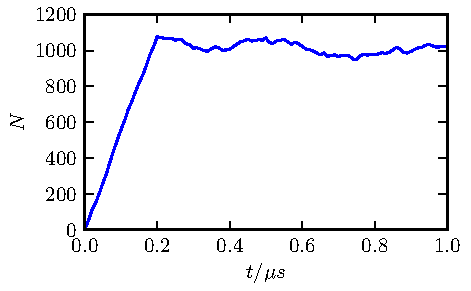
\includegraphics{ptcl_source/numPtclsVsT.pdf}
\end{center}
\caption{Number of particles in simulation domain as a function
of time.}
\end{figure}

\begin{figure}
\begin{center}
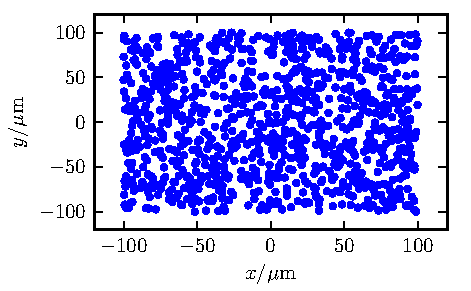
\includegraphics{ptcl_source/density.pdf}
\end{center}
\caption{Uniform density.}
\end{figure}

\begin{figure}
\begin{center}
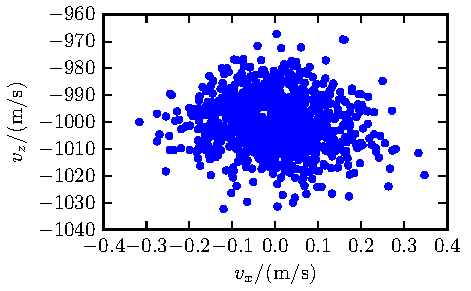
\includegraphics{ptcl_source/velocity_distribution.pdf}
\end{center}
\caption{Uniform density.}
\end{figure}


\subsection{Decay of the cavity field}

Decay and noise dynamics.  Also steady state fluctuations.


\subsection{Coherent evolution of coupled atom-field system}

Demonstrate Rabi oscillations with the correct Rabi frequency.


\subsection{Convergence study}


\section{TODO list}

\subsection{Near term}

\subsubsection{Get rid of Ring Buffer for particles {\bf [done]}}

The idea of the ring buffer data structure was to make it cheap
to add and remove particles from the simulation.  However, this
unduly penalizes other parts of the simulation that are
relatively more expensive.  In particular, it prevents
vectorization of many important loops.  In addition it makes much
of the code more complicated and leads to ambiguities where it is
not immediately apparent whether an array is a ring buffer or an
array.  Also, this is not needed for many simulations that don't
insert / remove particles frequently.

Removal and insertion of particles are affected by this change.
Particles should be inserted at the front of arrays (this
involves a \verb~memmove~; the only additional cost of using
arrays rather than a ring buffer) and particles should be deleted
from the end using a BSP similar to what's done in the ring
buffer implementation at the front.


\subsubsection{Need to scatter field amplitudes from rank 0 {\bf
[done]}}

Strictly speaking this is not needed as long as the field evolves
identically on each node (e.g.\ in the absence of noise in the
field equations).  But as soon as we add noise the field
amplitudes evolve differently on each node and only one of them
is the true amplitude.  We can still evolve the fields using the
same equations on each processor (as long as that's not too much
work) to simplify the control flow.  I.e.\ no need to add 
\verb~if (!rank) { ... }~ around the field updates.  The
amplitudes on ranks other than zero simply get overwritten.


\subsubsection{Parallel initialization of random number
generation {\bf [done]}}

The \verb~sprng~ library needs to be compiled and included
differently depending on whether it is used with MPI\@.


\subsubsection{Noise of the cavity field}

The Langevin noise terms give rise to the finite linewidth.


\subsubsection{Need better configurability from the command line}

Currently, configuration is done entirely via command line
options.  This is becoming pretty unwieldy.  As we're adding more
flexibility to  the code base problems are only going to
increase.  Options include a declarative configuration language
(xml, json, yaml) or bindings to a scripting language (python or
guile).


\subsubsection{Uniform mode function}

 Primarily for unit tests.


\subsubsection{Particle sources for initialization}


\subsubsection{More types of particle sources}


\subsection{Down the road}

The following are things we wish to tackle in the future.


\subsubsection{Photon scattering physics} This is going to be a big
one.  Adding this capability will allow us to do repumping among
other things.


\subsubsection{Trapping potential for atoms}


\subsubsection{Multimode fields} We will still focus on the case
of a small number of modes.


\end{document}

% vim: nocindent tw=65 spell

